\documentclass[12pt,a4paper]{article}
\usepackage[utf8]{inputenc}
\usepackage{amsmath}
\usepackage{amsfonts}
\usepackage{amssymb}
\usepackage[MeX]{polski}
\usepackage{graphicx}
\usepackage{hyperref}
\usepackage{algorithm}
\usepackage{algpseudocode}
\usepackage{float}
\usepackage{listings}

\floatname{algorithm}{Algorytm}
\newcommand{\algorithmname}{Algorytm}
\renewcommand\thesection{\arabic{section}}
\author{Mateusz Miotk 195025}
\title{Zgłębianie danych - Raport z projektu}


\begin{document}
\maketitle
\newpage
\tableofcontents
\newpage

\section[Treść projektu] {Treść projektu}
Przeprowadzić analizę opinii (sentiment mining) użytkowników Twittera na temat 
budzący różne emocje: polityka, politycy (dla kilku – zrobić sondaż) lub bieżące 
wydarzenia. Wykorzystać pakiet R z doinstalowaną paczką twitteR lub program 
RapidMiner z rozszerzeniem TextMining. Sklasyfikować kilkaset/tysiecy tweetów jako 
negatywne i pozytywne (w różnym stopniu) na podstawie odpowiednio dobranej listy 
słów kluczowych. Nastepnie przanalizuj i zinterpretuj wyniki: częstość występowania 
opinii, średnią, odchylenie standardowe, wykres/histogram.
\section[Krótki wstęp dotyczący projektu i jego zastosowania] {Wstęp}
Semantic analysis inaczej też nazywana opinion mining jest to obliczeniowe przetwarzanie emocji, opinii, postaw, ocen itd. na podstawie tekstów, którymi mogą być między innymi: wywiady, blogi, dyskusje, wiadomości, komentarze itd. \\
Metoda ta w ogólności polega na podziału opinii na trzy podstawowe grupy: pozytywne,neutralne oraz negatywne. Ma to ogromny wpływ w biznesie, ponieważ na przykład dzięki opiniom klientów danego produktu możemy stwierdzić czy produkt ten spełnia oczekiwania, jakie założyliśmy.\\
W raporcie zostanie pokazane wykorzystanie tej techniki, opierając się na komentarzach znanego medium społecznościowego jakim jest twitter, badając emocje dotyczące różnych aktualnych wydarzeń ze świata. \\
\section[Narzędzia jakie zostały użyte] {Narzędzia jakie zostały użyte.}
Eksperyment został wykonany na systemie operacyjnym Ubuntu 14.04 x64 za pomocą pakietu statystycznego R który można pobrać ze strony: \url{http://www.r-project.org/}.\\
Poza tym będziemy potrzebować pakietu \textbf{libcurl4-openssl-dev} który możemy zainstalować za pomocą terminala poleceniem \textbf{sudo apt-get install libcurl4-openssl-dev}. Pakiet ten jest nam potrzebny do połączenia pakietu R z twitterem. 

\section[Schemat algorytmu wykonania sentiment analysis] {Schemat algorytmu wykonania sentiment analysis}
Badanie opinii będzie ogólnie wyglądało następująco: \\

\begin{algorithm}
\caption{Schemat algorytmu wykonania sentiment analysis}
\begin{algorithmic}[1]

\Procedure{sentimentAnalysisTwitter}{}
    \State Dokonaj połączenia pakietu R z twitterem.
    \State Pobierz dane z twittera.
    \State Dokonaj wyczyszczenia oraz poprawienia otrzymanych danych poprzez wyrażenia regularne.
    \State Wykonaj funkcję sentiment dla wyczyszczonych danych.
\EndProcedure
\end{algorithmic}
\end{algorithm}

\section[Opis poszczególnych metod algorytmu]{Opis poszczególnych metod algorytmu}
\subsection[Połączenie pakietu R z twitterem] {Połączenie pakietu R z twitterem}
Do połączenia pakietu R z twitterem będziemy musieli zainstalować następujące dodatkowe pakiety w pakiecie R: 
\begin{itemize}
\item RCurl - pakiet, który pozwala nam połączyć pakiet R ze stroną http//: lub ftp//:
\item ROAuth - pakiet zawierający interfejs połączenia aplikacji wedle specyfikacji OAuth 1.0 .
\item bitops - pakiet zawierający bitowe operację, które możemy wykonywać na wektorach.
\item digest - pakiet zawierający implementację funkcji skrotów MD5, sha1 itd. 
\item rjson - pakiet pozwalający czytać/zapisywać w formacie json. 
\item plyr - pakiet zawierający mnóstwo funckji, służący do rozwiązywania wielkich problemów poprzez dzielenie je na podproblemy. 
\item stringr - pakiet zawierający ulepszone funkcję, które możemy wykonywać na napisach.
\item twitteR - pakiet zawierający funkcję, poprzez które możemy wykorzystywać twittera w pakiecie R.
\end{itemize}

Nie będziemy korzystać z wszystkich wyżej wymienionych pakietów, aczkolwiek są one wymagane do uruchomienia pakietu twitteR. 
Aby zainstalować pakiet w języku R należy w konsoli wpisać polecenie: \\ \textbf{install.packages$\left("nazwa"\right)$.}

Kolejnym krokim jakim musimy wykonać jest stworzenie aplikacji na stronie twitter.com. \\
Aby tego dokonać należy wejść na stronę \url{https://dev.twitter.com/} i zalogować się poprzez konto na twitterze. Następnie należy wejść na stronę \url{https://apps.twitter.com/} i stworzyć  aplikacje poprzez kliknięcie na przycisk \textbf{Create a new app}.

\begin{figure}[H]
\begin{center}
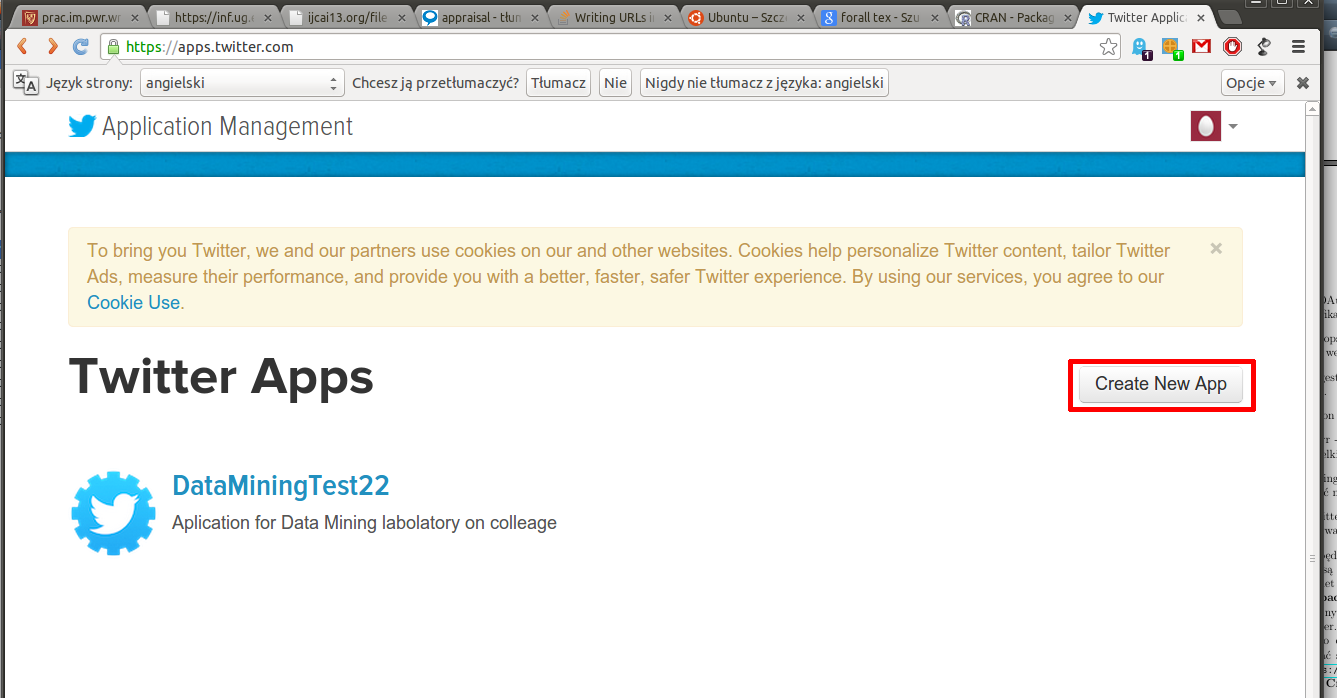
\includegraphics[scale=0.2]{pictures/Twitter1.png}
\caption{Tworzenie nowej aplikacji w twitterze.}
\end{center}
\end{figure}
Następnie należy wypełnić pola obowiązkowe i utworzyć aplikację: 
\begin{figure}[H]
\begin{center}
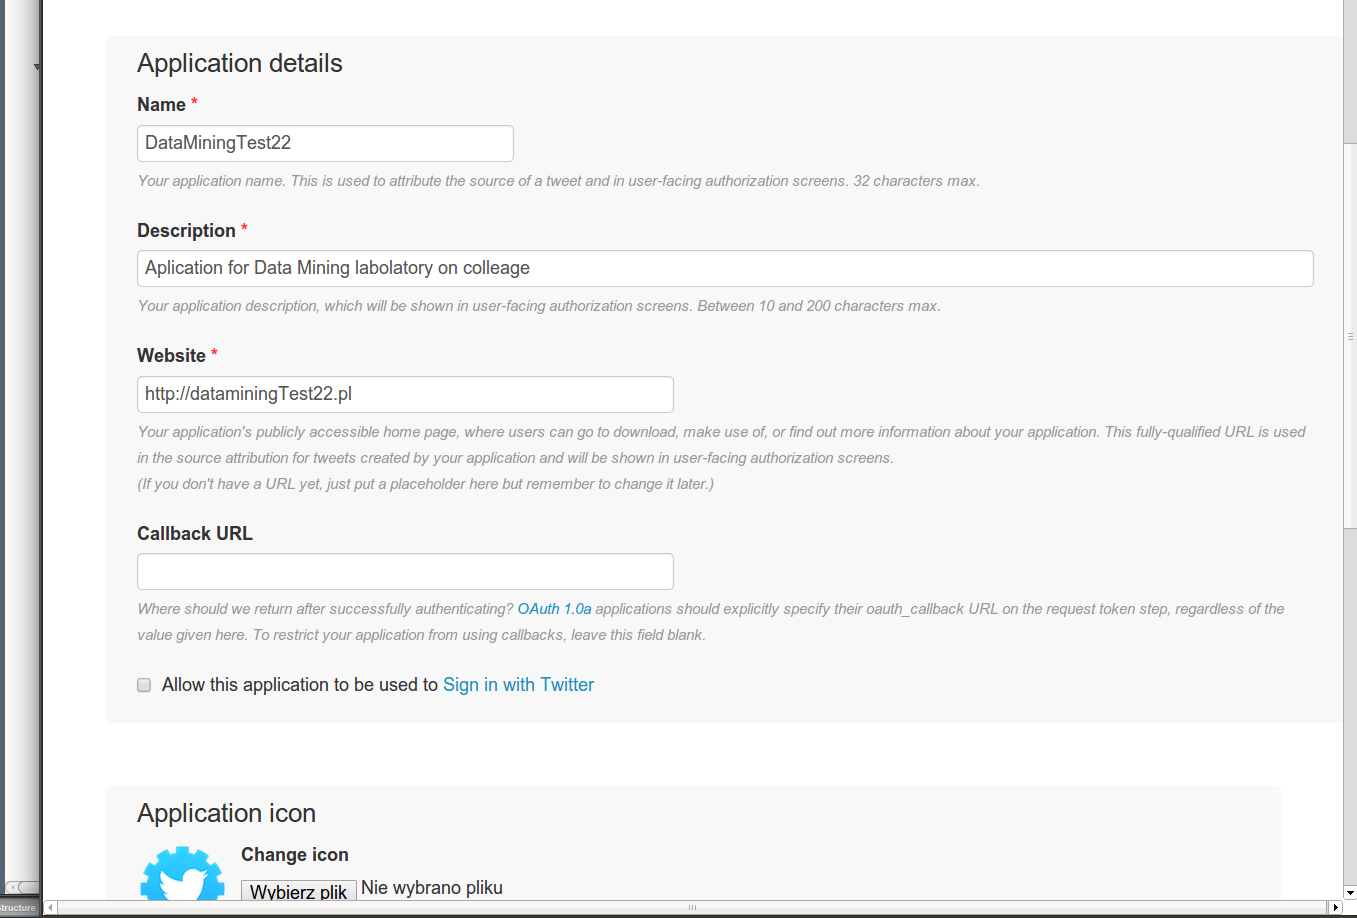
\includegraphics[scale=0.2]{pictures/Twitter2.png}
\caption{Opis tworzonej aplikacji}
\end{center}
\end{figure}

Po utworzeniu aplikacji wchodzimy do niej, otwieramy zakładkę \textbf{Details} i kopiujemy następujące elementy: 
\begin{figure}[H]
\begin{center}
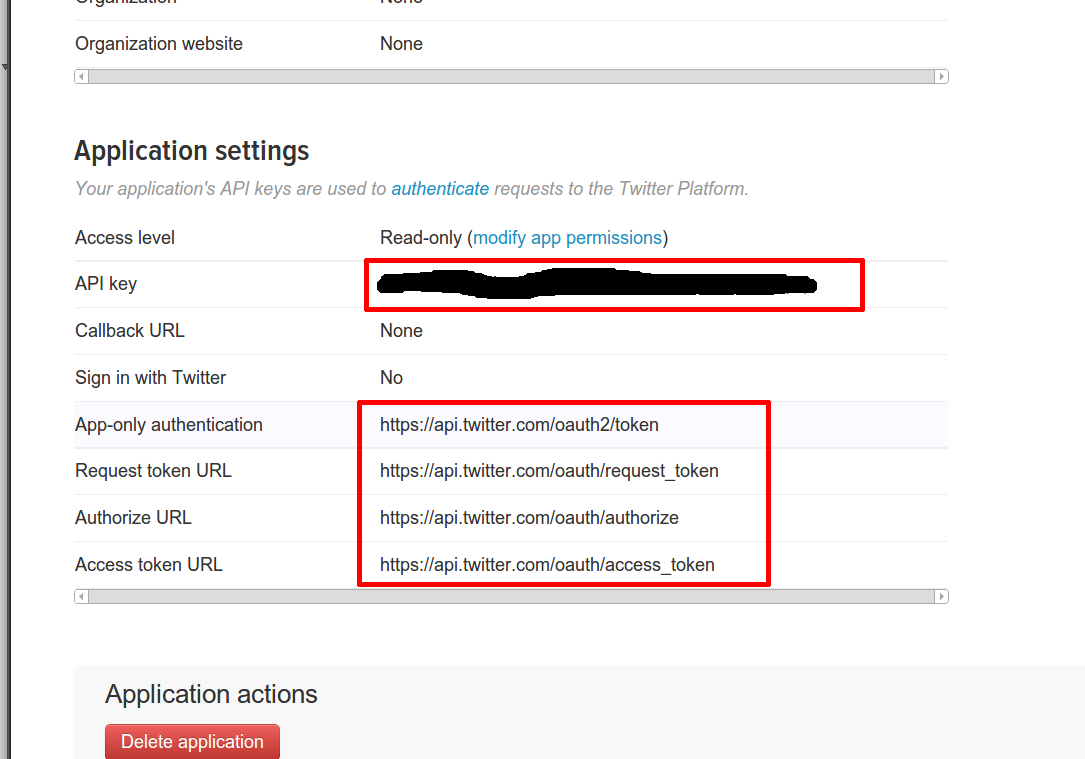
\includegraphics[scale=0.2]{pictures/Twitter3.png}
\caption{Potrzebne elementy z naszej twitterowej aplikacji}
\end{center}
\end{figure}
Ostatnią rzecz jaką będziemy potrzebować to \textbf{apiSecret}, który znajdziemy w zakładce \textbf{API Keys}.
\begin{figure}[H]
\begin{center}
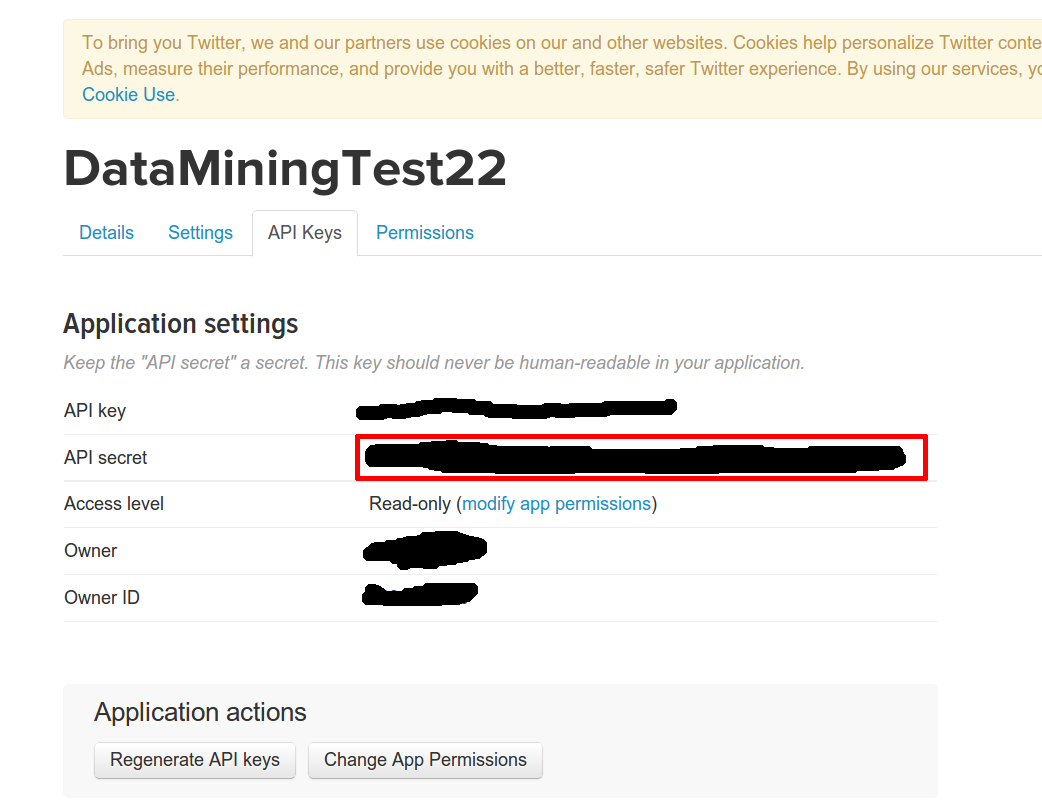
\includegraphics[scale=0.2]{pictures/Twitter4.png}
\caption{API secret naszej aplikacji}.
\end{center}
\end{figure}

Mając wszystkie te rzeczy możemy przystąpić do napisania kodu w języku R, która połączy się z twitterem poprzez naszą utworzoną aplikację.

\begin{figure}[H]
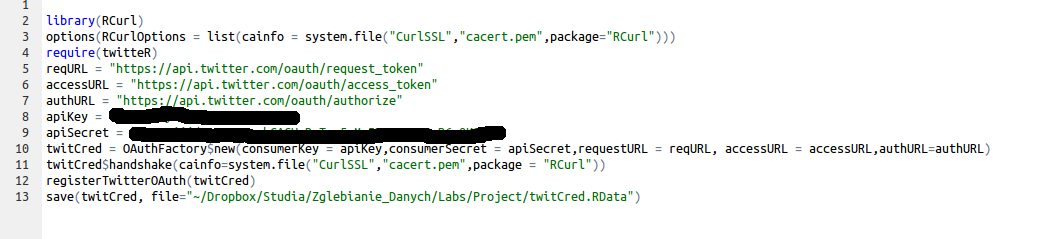
\includegraphics[scale=0.45]{pictures/Code1.png}
\caption{Kod autoryzujący pakiet R z naszą aplikacja w twitterze.}
\end{figure}

Polecenie \textbf{library} ładuje pakiet do środowiska. Polecenie \textbf{options} pobiera standardowy certyfikat cacert.pem do wykonania autoryzacji aplikacji. Polecenie \textbf{require} działa tak samo jak library z tą różnicą, że ładuje wszystkie dodatkowe potrzebne pakiety do środowiska. Polecenie \textbf{OAuthFactory} łączy środowisko pakietu R z naszą aplikacją twitterową, która jest zaakceptowana poprzez polecenie \textbf{registerTwitterOAuth}. Polecenie \textbf{save} zapisuje nam plik, dzięki któremu będziemy mogli w każdej chwili połączyć się z naszą aplikacją używając wyłącznie polecenie \textbf{registerTwitterOAuth}. \\
Gdy wywołamy powyższy skrypt to środowisko pakietu R wygeneruje nam link dzięki któremu będziemy musieli autoryzować naszą aplikację stworzoną na twitterze. Aby tego dokonać należy skopiować link oraz kliknąć przycisk \textbf{Authorize app}
\begin{figure}[H]
\begin{center}
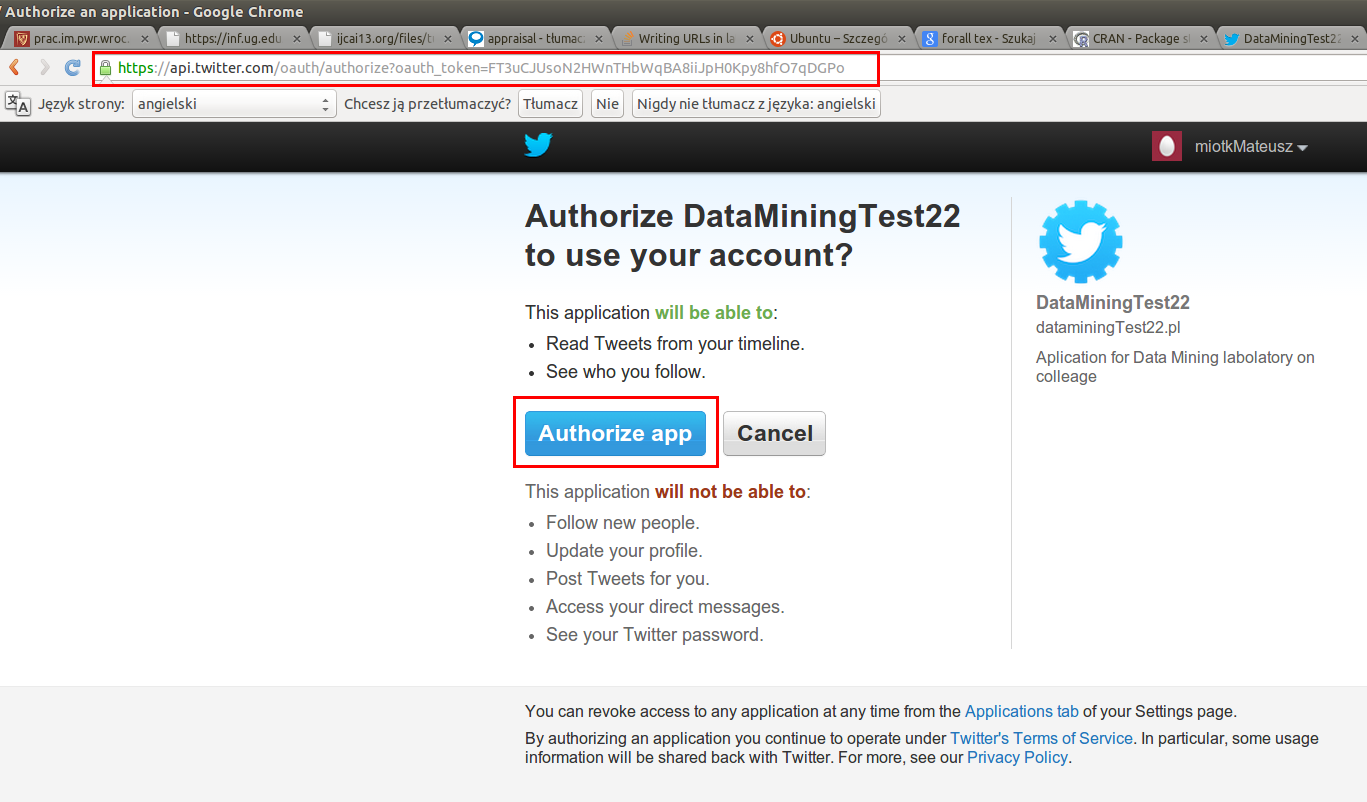
\includegraphics[scale=0.25]{pictures/Twitter5.png}
\caption{U góry otrzymany link z konsoli R, poniżej przycisk autoryzujący aplikację.}
\end{center}
\end{figure}

Po kliknięciu przycisku \textbf{Authorize app} wyświetli się nam numer pin który będziemy musieli wpisać w konsoli środowiska pakietu R.
\begin{figure}[H]
\begin{center}
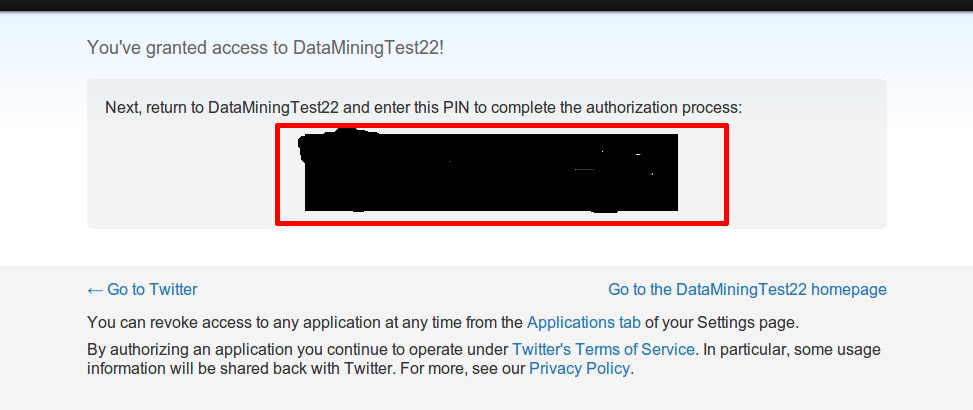
\includegraphics[scale=0.25]{pictures/Twitter6.png}
\caption{Kod pin autoryzujący naszą aplikację z twitterem}
\end{center}
\end{figure}

\begin{figure}[H]
\begin{center}
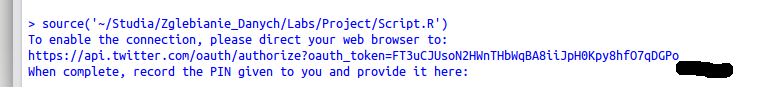
\includegraphics[scale=0.5]{pictures/Console1.png}
\caption{Wpisanie pinu do konsoli pakietu R}
\end{center}
\end{figure}


\subsection[Pobieranie danych z twittera]{Pobieranie danych z twittera}
Jeśli już mamy aplikację zautoryzowaną z twitterem możemy przejść do przeglądania tweetów na dany temat. 
\begin{figure}[H]
\begin{center}
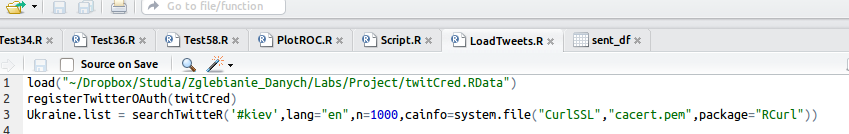
\includegraphics[scale=0.5]{pictures/Code2.png}
\caption{Połączenie się z twitterem oraz przykładowa funkcja wyszukująca tweety.}
\end{center}
\end{figure}

Wyszukiwanie tweetów weykonuje funckja \textbf{searchTwitteR}. Jej parametrami są w naszym przypadku ciąg jaki szukamy, w jakim języku, ile chcemy uzyskać tweetów oraz certyfikat przez który się łączymy z api Twittera. \\
Uzyskane dane wyglądają obecnie następująco: \\
\begin{figure}[H]
\begin{center}
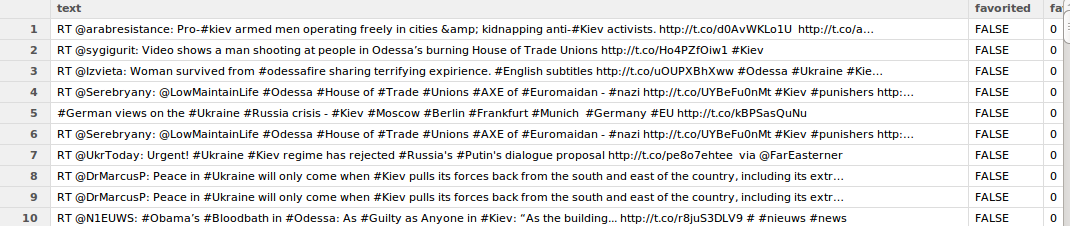
\includegraphics[scale=0.45]{pictures/Data1.png}
\caption{Przykładowe dane pobrane za pomocą paczki twitteR.}
\end{center}
\end{figure}

Aby otrzymać powyższą tabelę z danymi musimy te dane przerobić z naszej listy do obiektu typu \textbf{data frame}. Wykonujemy to poleceniem:\\ \textbf{twListToDF$(nazwa)$} \\
Otrzymane tweety zawsze możemy zapisać w postaci \textbf{.csv} używając polecenia: \\
\textbf{write.csv$($obiekt,ścieżka,row.names=F$)$}.

\subsection[Wyczyszczenie i uporządkowanie danych za pomocą wyrażeń regularnych]{Wyczyszczenie i uporządkowanie danych za pomocą wyrażeń regularnych}
Uzyskane powyższe tweety są bardzo nieeleganckie. Zawierają one znaki, które powodują że w algorytmie sentiment nie będą one brane pod uwagę. Musimy oczyścić otrzymane tweety za pomocą wyrażeń regularnych. Dokonujemy tego poprzez wywołanie następującego kodu: \\
\begin{figure}[H]
\begin{center}
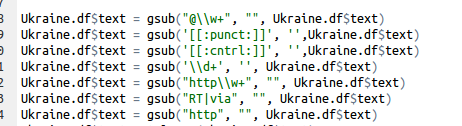
\includegraphics[scale=0.5]{pictures/Code3.png}
\caption{Polecenia służące wyczyszczeniu i uporządkowaniu danych z twittera.}
\end{center}
\end{figure}

Tak więc aby oczyścić nasze tweety za pomocą wyrażeń regularnych używamy funkcji \textbf{gsub}. Funkcja \textbf{gsub} zastępuje wyrażenia, który jest podany jako pierwszy argument wzorcem podanym jako drugi argument. Jako trzeci argument wymaga on podania danych na których ma wykonać zamianę. Pierwszy wiersz pozbywa się nazw loginów, z którego otrzymaliśmy dany tweet. 
Wyrażenie \textbf{$[[:punct:]]$} wyszukuje wszystkie znaki specjalne i punktowalne typu @ [ ] itd. Wyrażenie \textbf{$[[:cntl:]]$} wyszukuje wszyskie znaki kontrolne. Pozostałe wyrażenia są jasne do zrozumienia. \\
Jeśli wykonamy powyższe kroki na zbiorze naszych zebranych tweetów to otrzymamy już bardziej elegancką formę do przeczytania i wykonania sentiment analysis.

\begin{figure}[H]
\begin{center}
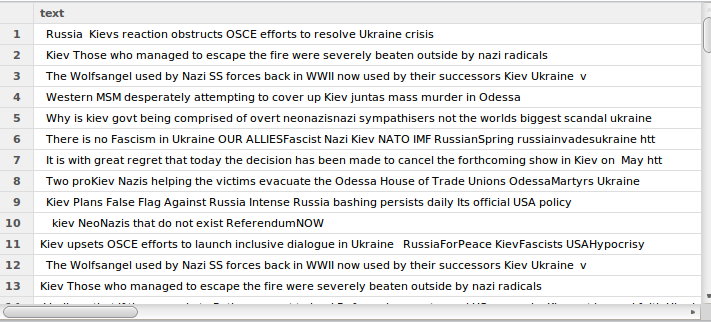
\includegraphics[scale=0.5]{pictures/Data2.png}
\caption{Wyczyszczone i uporządkowane dane z twittera.}
\end{center}
\end{figure}


\subsection[Funkcja sentiment]{Funkcja sentiment}
Mając tak przygotowane dane możemy przystąpić już teraz do realizacji sentiment analysis. Aby tego dokonać będziemy jeszcze potrzebować drobnych zmian w otrzymanych, przerobionych tekstach tekstach. Po pierwsze musimy zamienić wszystko na małe litery. Wykonujemy to za pomocą polecenia \textbf{tolower}. 
Następnie dla każdego otrzymanego tweeta dzielimy go na listę pojedyńczych słów. Dokonujemy tego za pomocą polecenia \textbf{strsplit}. 
Teraz wystarczy tylko dokonać porównania z listą pozytywnych oraz negatywnych słów. Dla języka angielskiego listę pozytywnych oraz negatywnych słów możemy ściągnąć ze strony \textbf{\url{http://www.cs.uic.edu/~liub/FBS/opinion-lexicon-English.rar}} \\
Używamy funkcji \textbf{match}, która obliczy nam pozycje podzielonych słów naszego tweeta w naszym słowniku słów pozytywnych i negatywnych. Jeśli dane słowo nie występuje w żadnym ze słowników otrzymuje ono wartość zero. \\
Aby otrzymać czy dana opinia jest pozytywna, neutralna czy negatywna wystarczy  wykonać odpowiednie działanie: 
\begin{center}
$ opinia = \sum ($pozytywne słowa$) - \sum ($negatywne słowa$) $ \\
\end{center}

Uzyskany wynik należy wówczas implementować następująco: \\
\[\mbox{sentiment analysis} \left \lbrace \begin{array}{cl}
pozytywna &~ opinion > 0 \\
neutralna &~ opinion=0 \\
negatywna &~ opinion < 0
\end{array} \right. \]
\begin{figure}[H]
\begin{center}
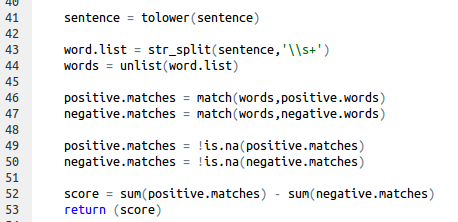
\includegraphics[scale=0.5]{pictures/Code6.png}
\caption{Implementacja funckji sentiment w pakiecie R}
\end{center}
\end{figure}


\section[Użycie sentiment analysis do analizy danych]{Użycie sentiment analysis do analizy danych}
Mając tak napisany program w pakiecie R rozważmy następujące doświadczenie: Weźmy sobie kilkaset tweetów dotyczące słów wzbudzający emocję. Niech będą nimi następujące słowa: narkotyki, alkohol, rasizm, małżeństwo, praca, samochód. Dokonamy sentiment analysis na  \textbf{500} tweetach zawierające powyższe nazwy. Obliczymy do tego histogram występowania wartości opinion oraz jakie ma ono odchylenie standardowe oraz średnią. Dzięki uzyskanym wynikom możemy stwierdzić jak dane słowo jest odbierane przez użytkowników twittera.\\
Tak więc dla danych słów uzyskaliśmy następujące wyniki: \\


\begin{table}[H]
\begin{tabular}{|c|c|c|c|c|c|}
\hline
Słowo & Pozytywne & Negatywne & Neutralne & Średnia  & Odchylenie \\
    \hline
    narkotyki & 91 & 178 & 231 & -0.21 & 1  \\
    alkohol & 141 & 104 & 255 & 0.13 & 1.07  \\
    rasizm & 16 & 406 & 78 & -1.24 & 0.96  \\
    małżeństwo & 159 & 244 & 97 & 0.04 & 1.29  \\
    praca & 421 & 12 & 67 & 1.24 & 1.1 \\
    samochód & 141 & 84 & 275 & 0.2 & 1.02  \\
    \hline
    
    \end{tabular}
\end{table}
Można było spodziewać się następujących wyników. Otóż najbardziej negatywnym słowem w naszym zestawieniu jest rasizm, zaś najbardziej pozytywnym praca. Zaskakujące są wyniki w słowie narkotyki gdzie bardzo dużo opinii jest sklasyfikowane jako neutralne. Drugim zaskoczeniem jest przewaga negatywnych opinii występujące w słowie: małżeństwo. \\
Przejdźmy do histogramów częstości dla danych słów: \\

\begin{center}
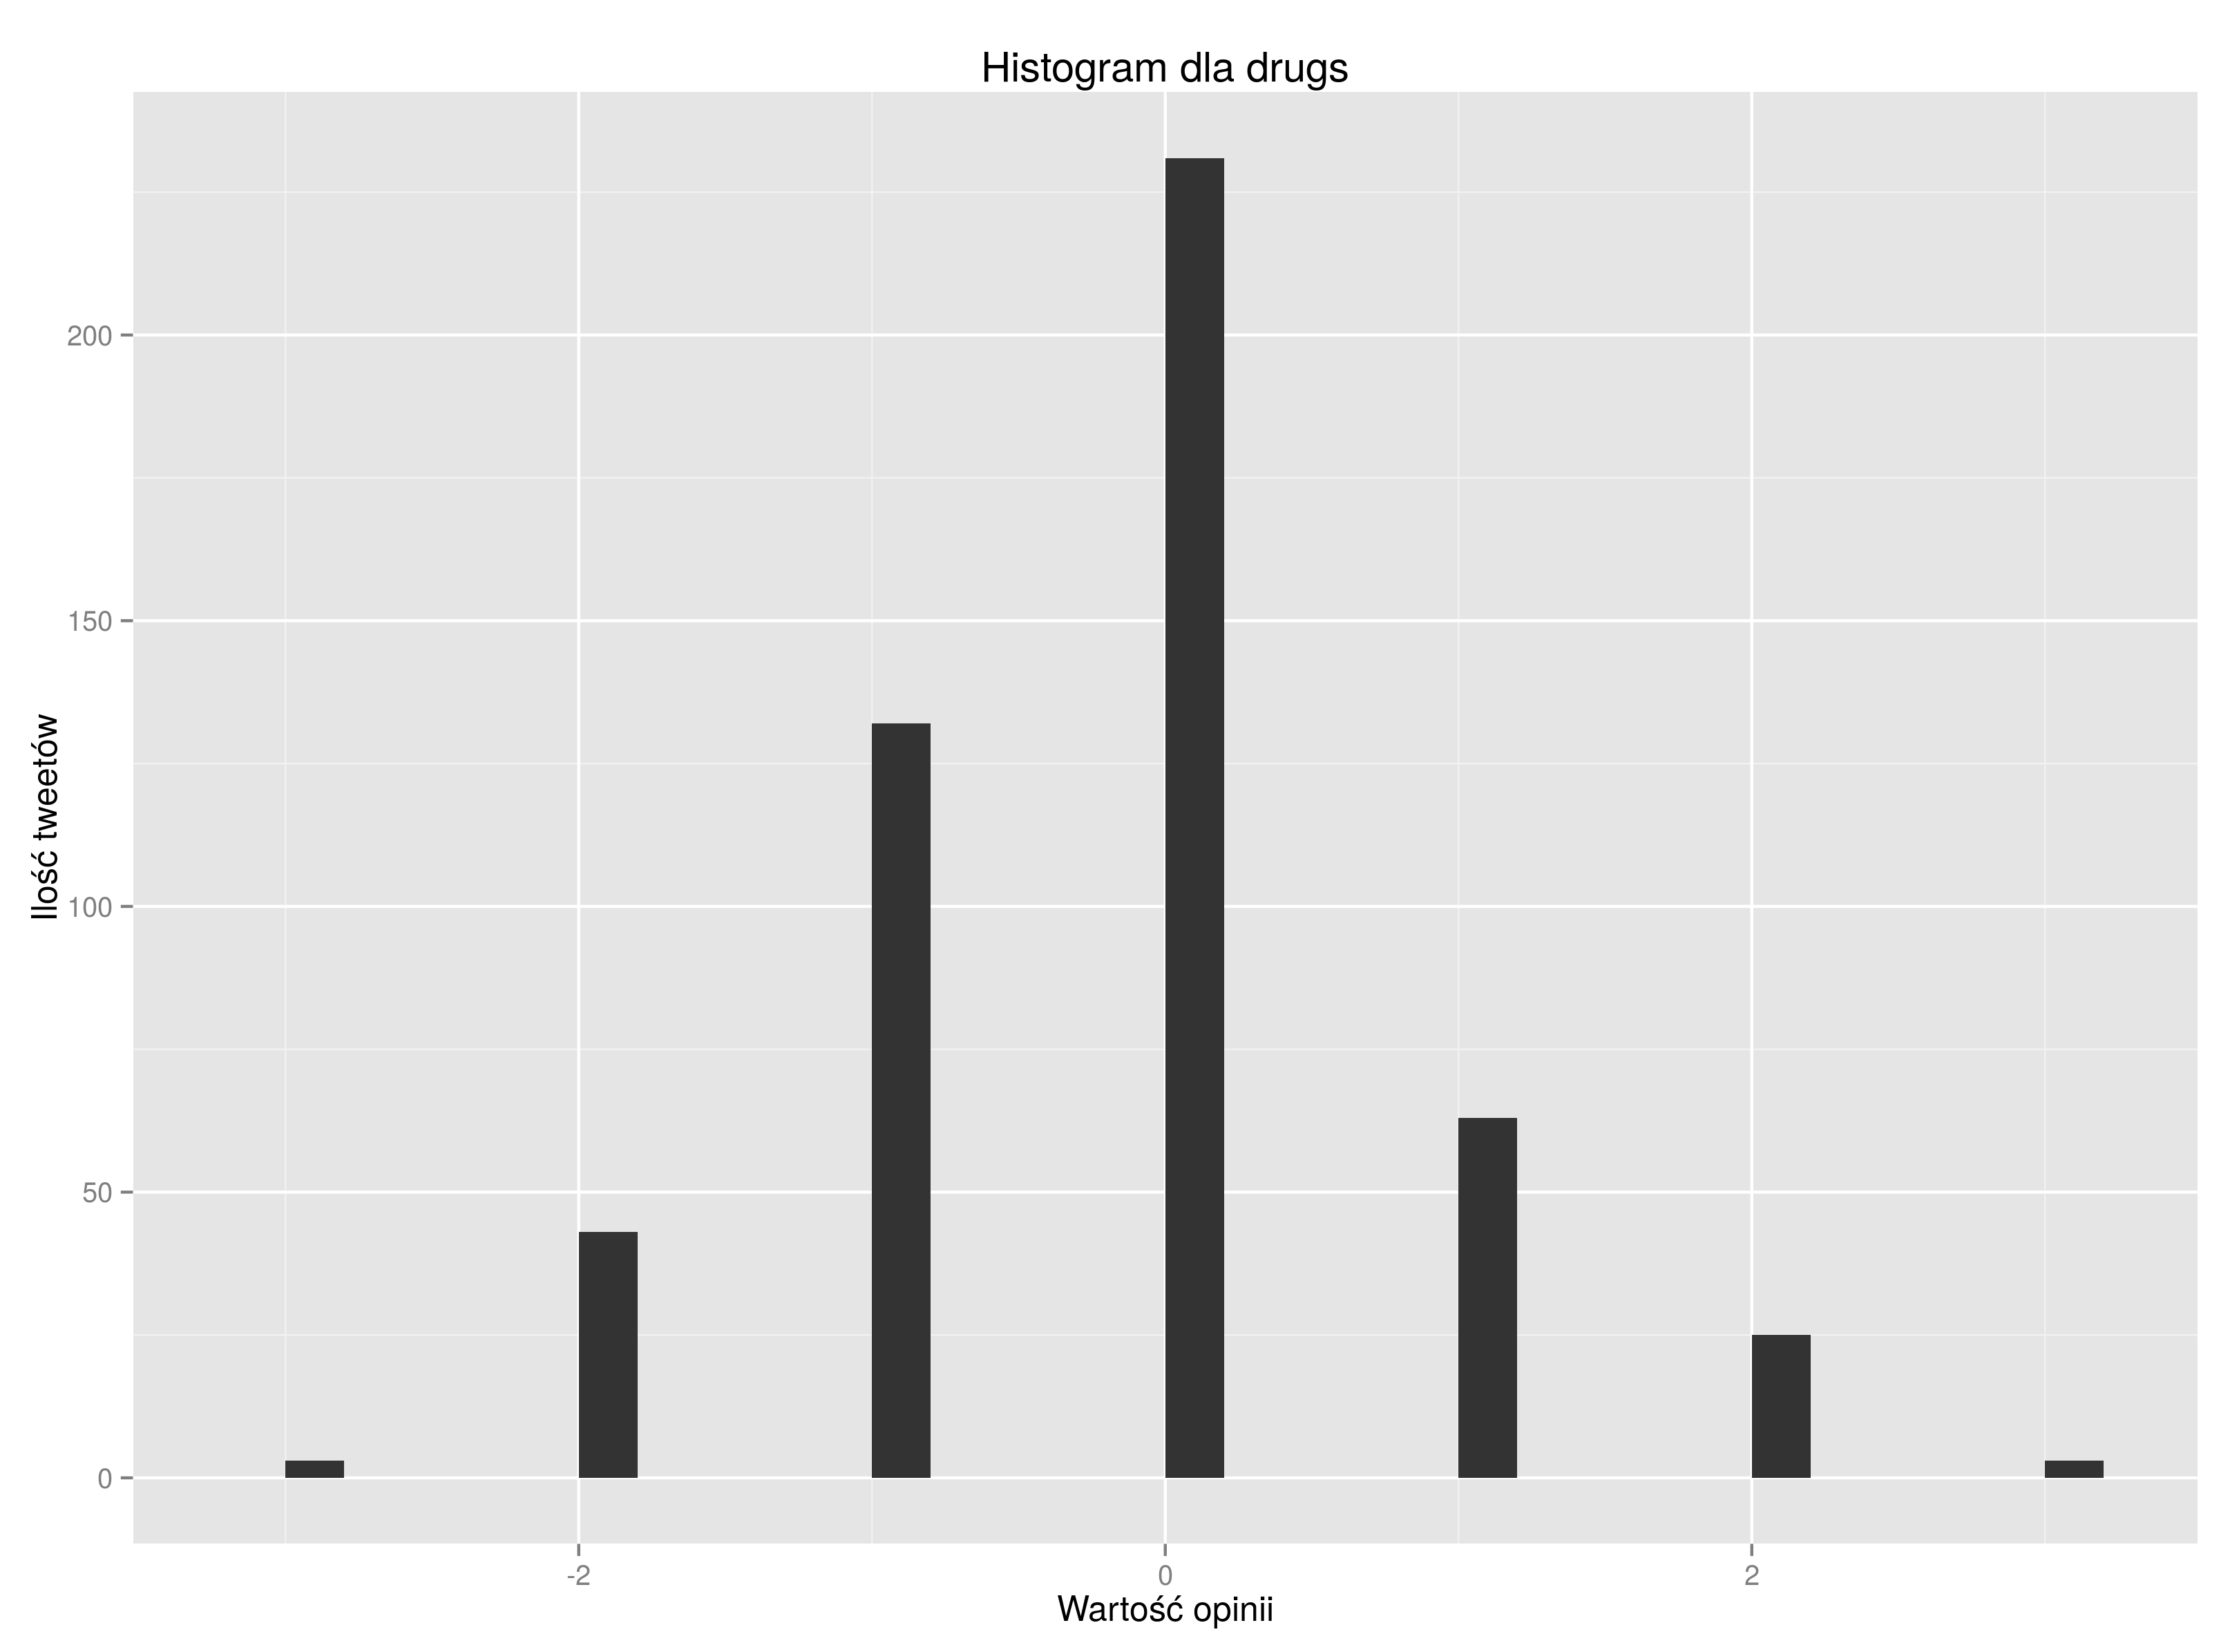
\includegraphics[scale=0.35]{pictures/Histdrugs.png}
\end{center}

\begin{center}
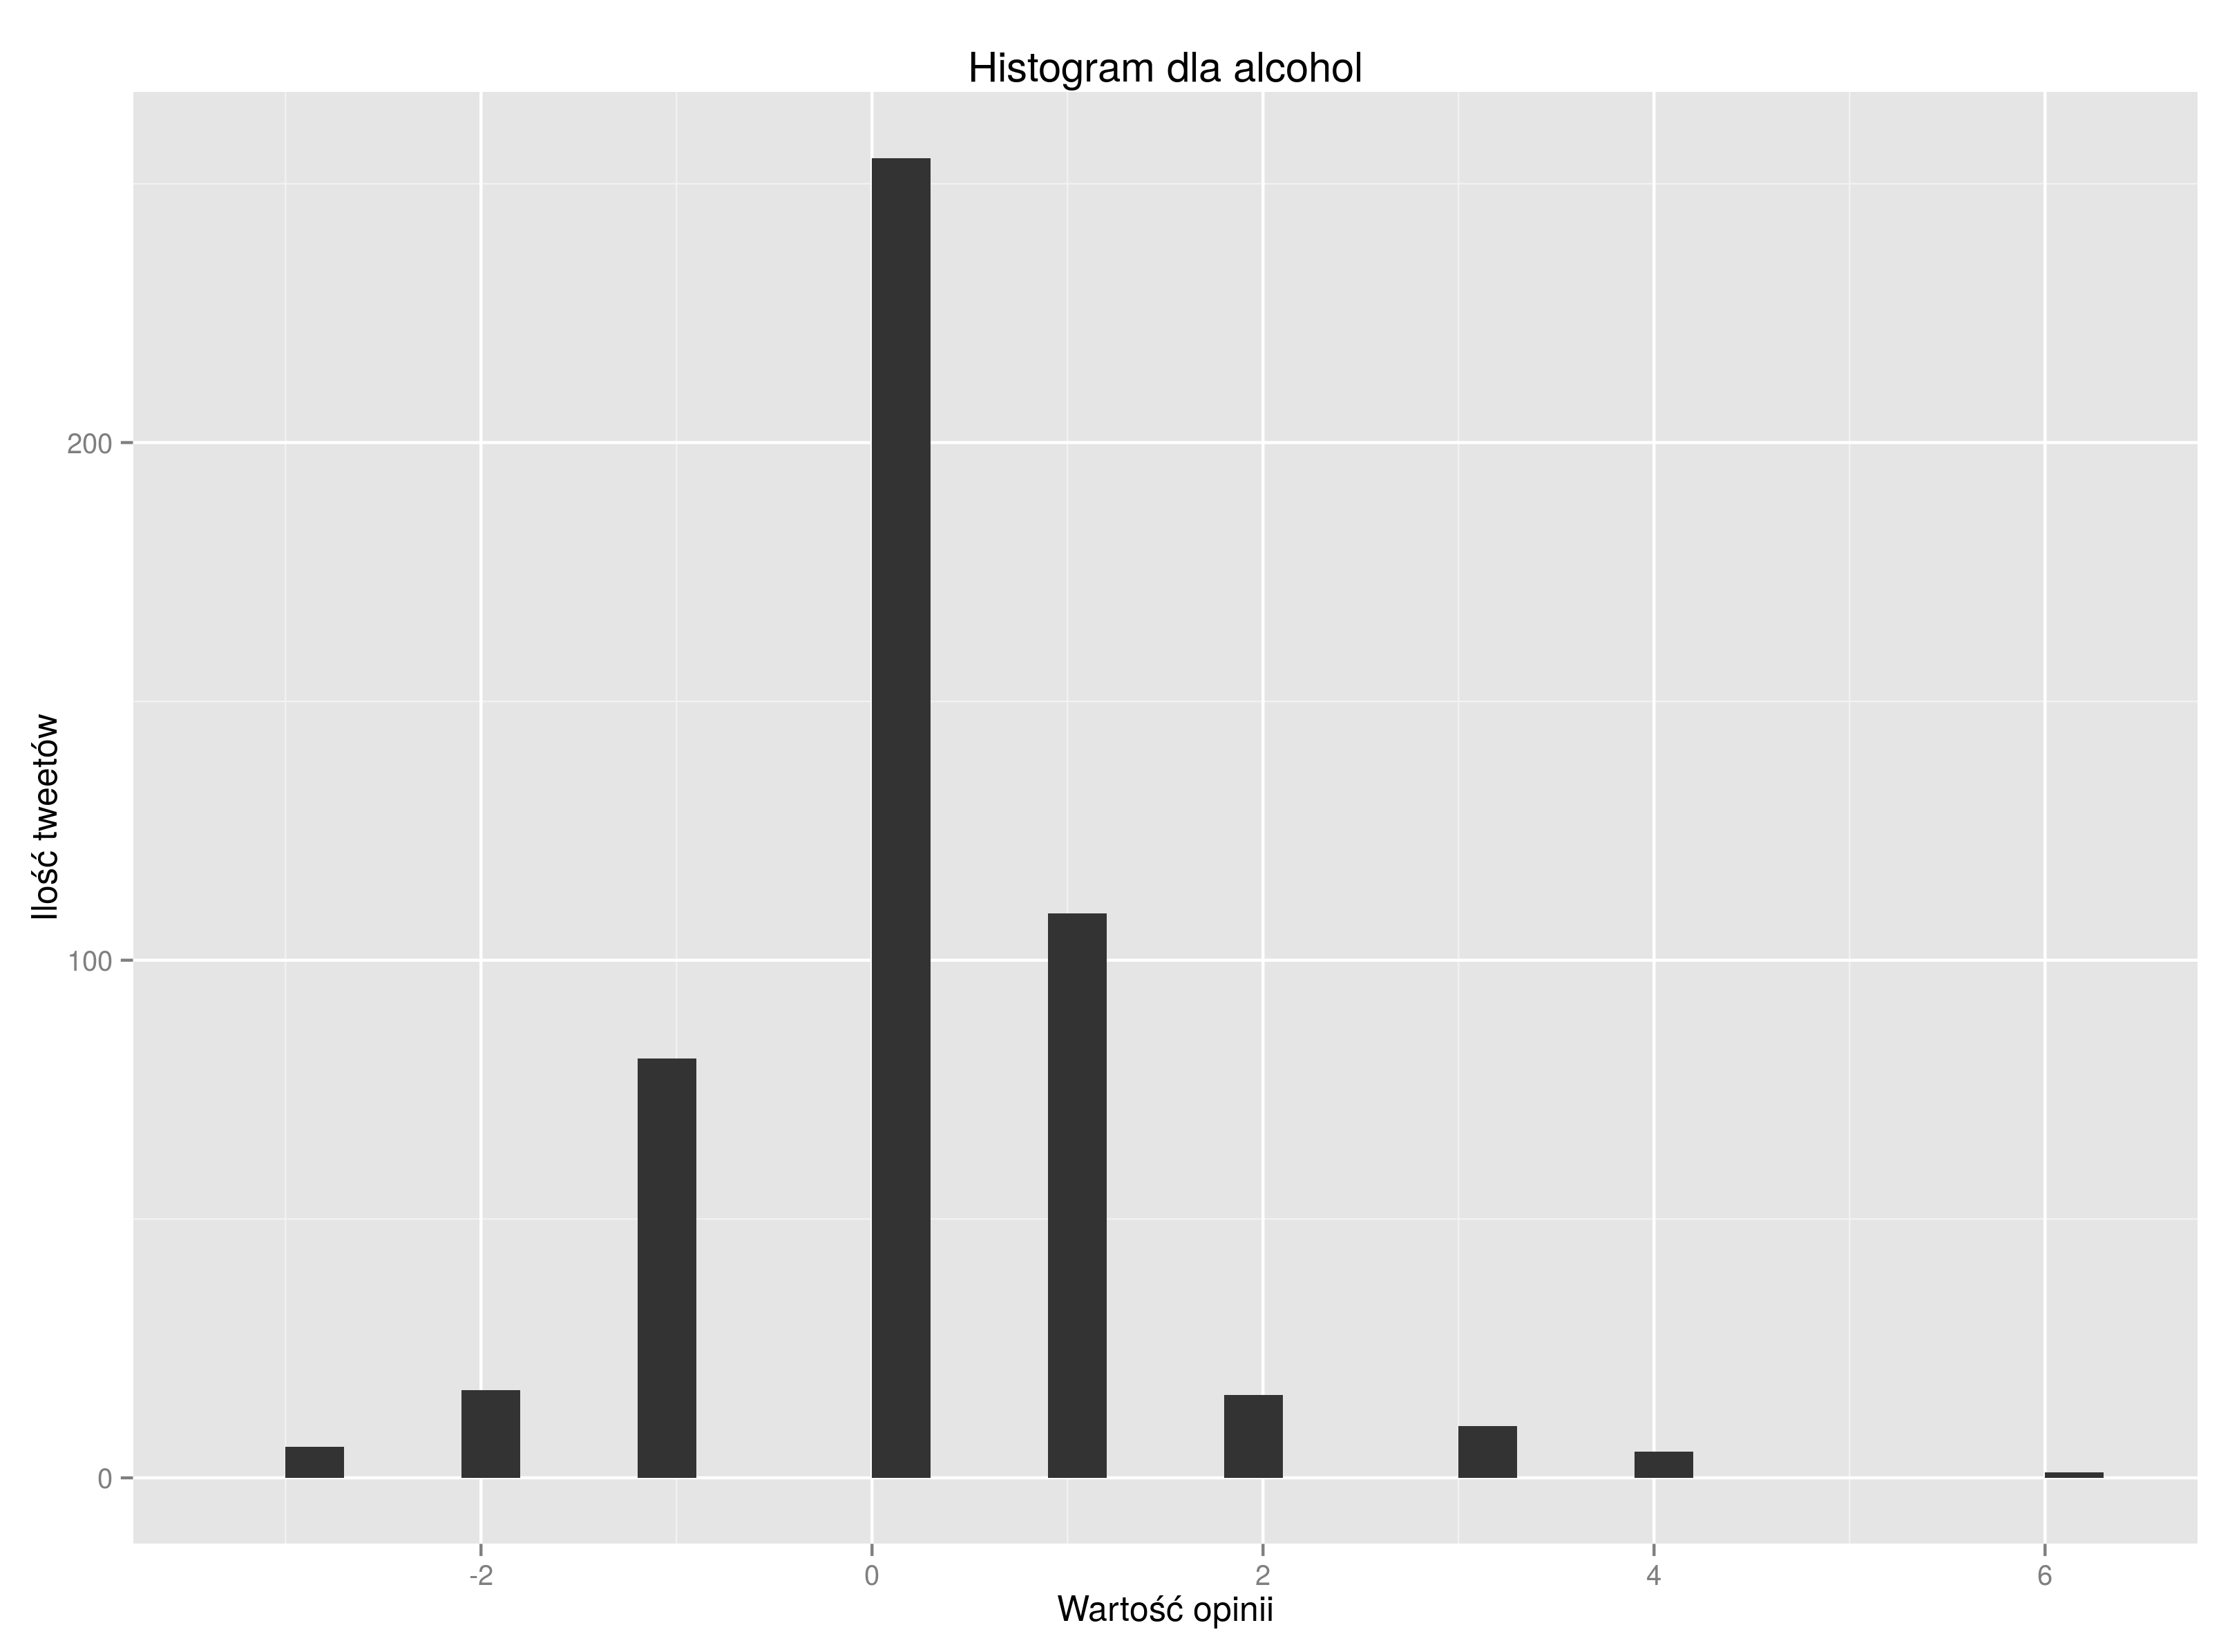
\includegraphics[scale=0.35]{pictures/Histalcohol.png}
\end{center}

\begin{center}
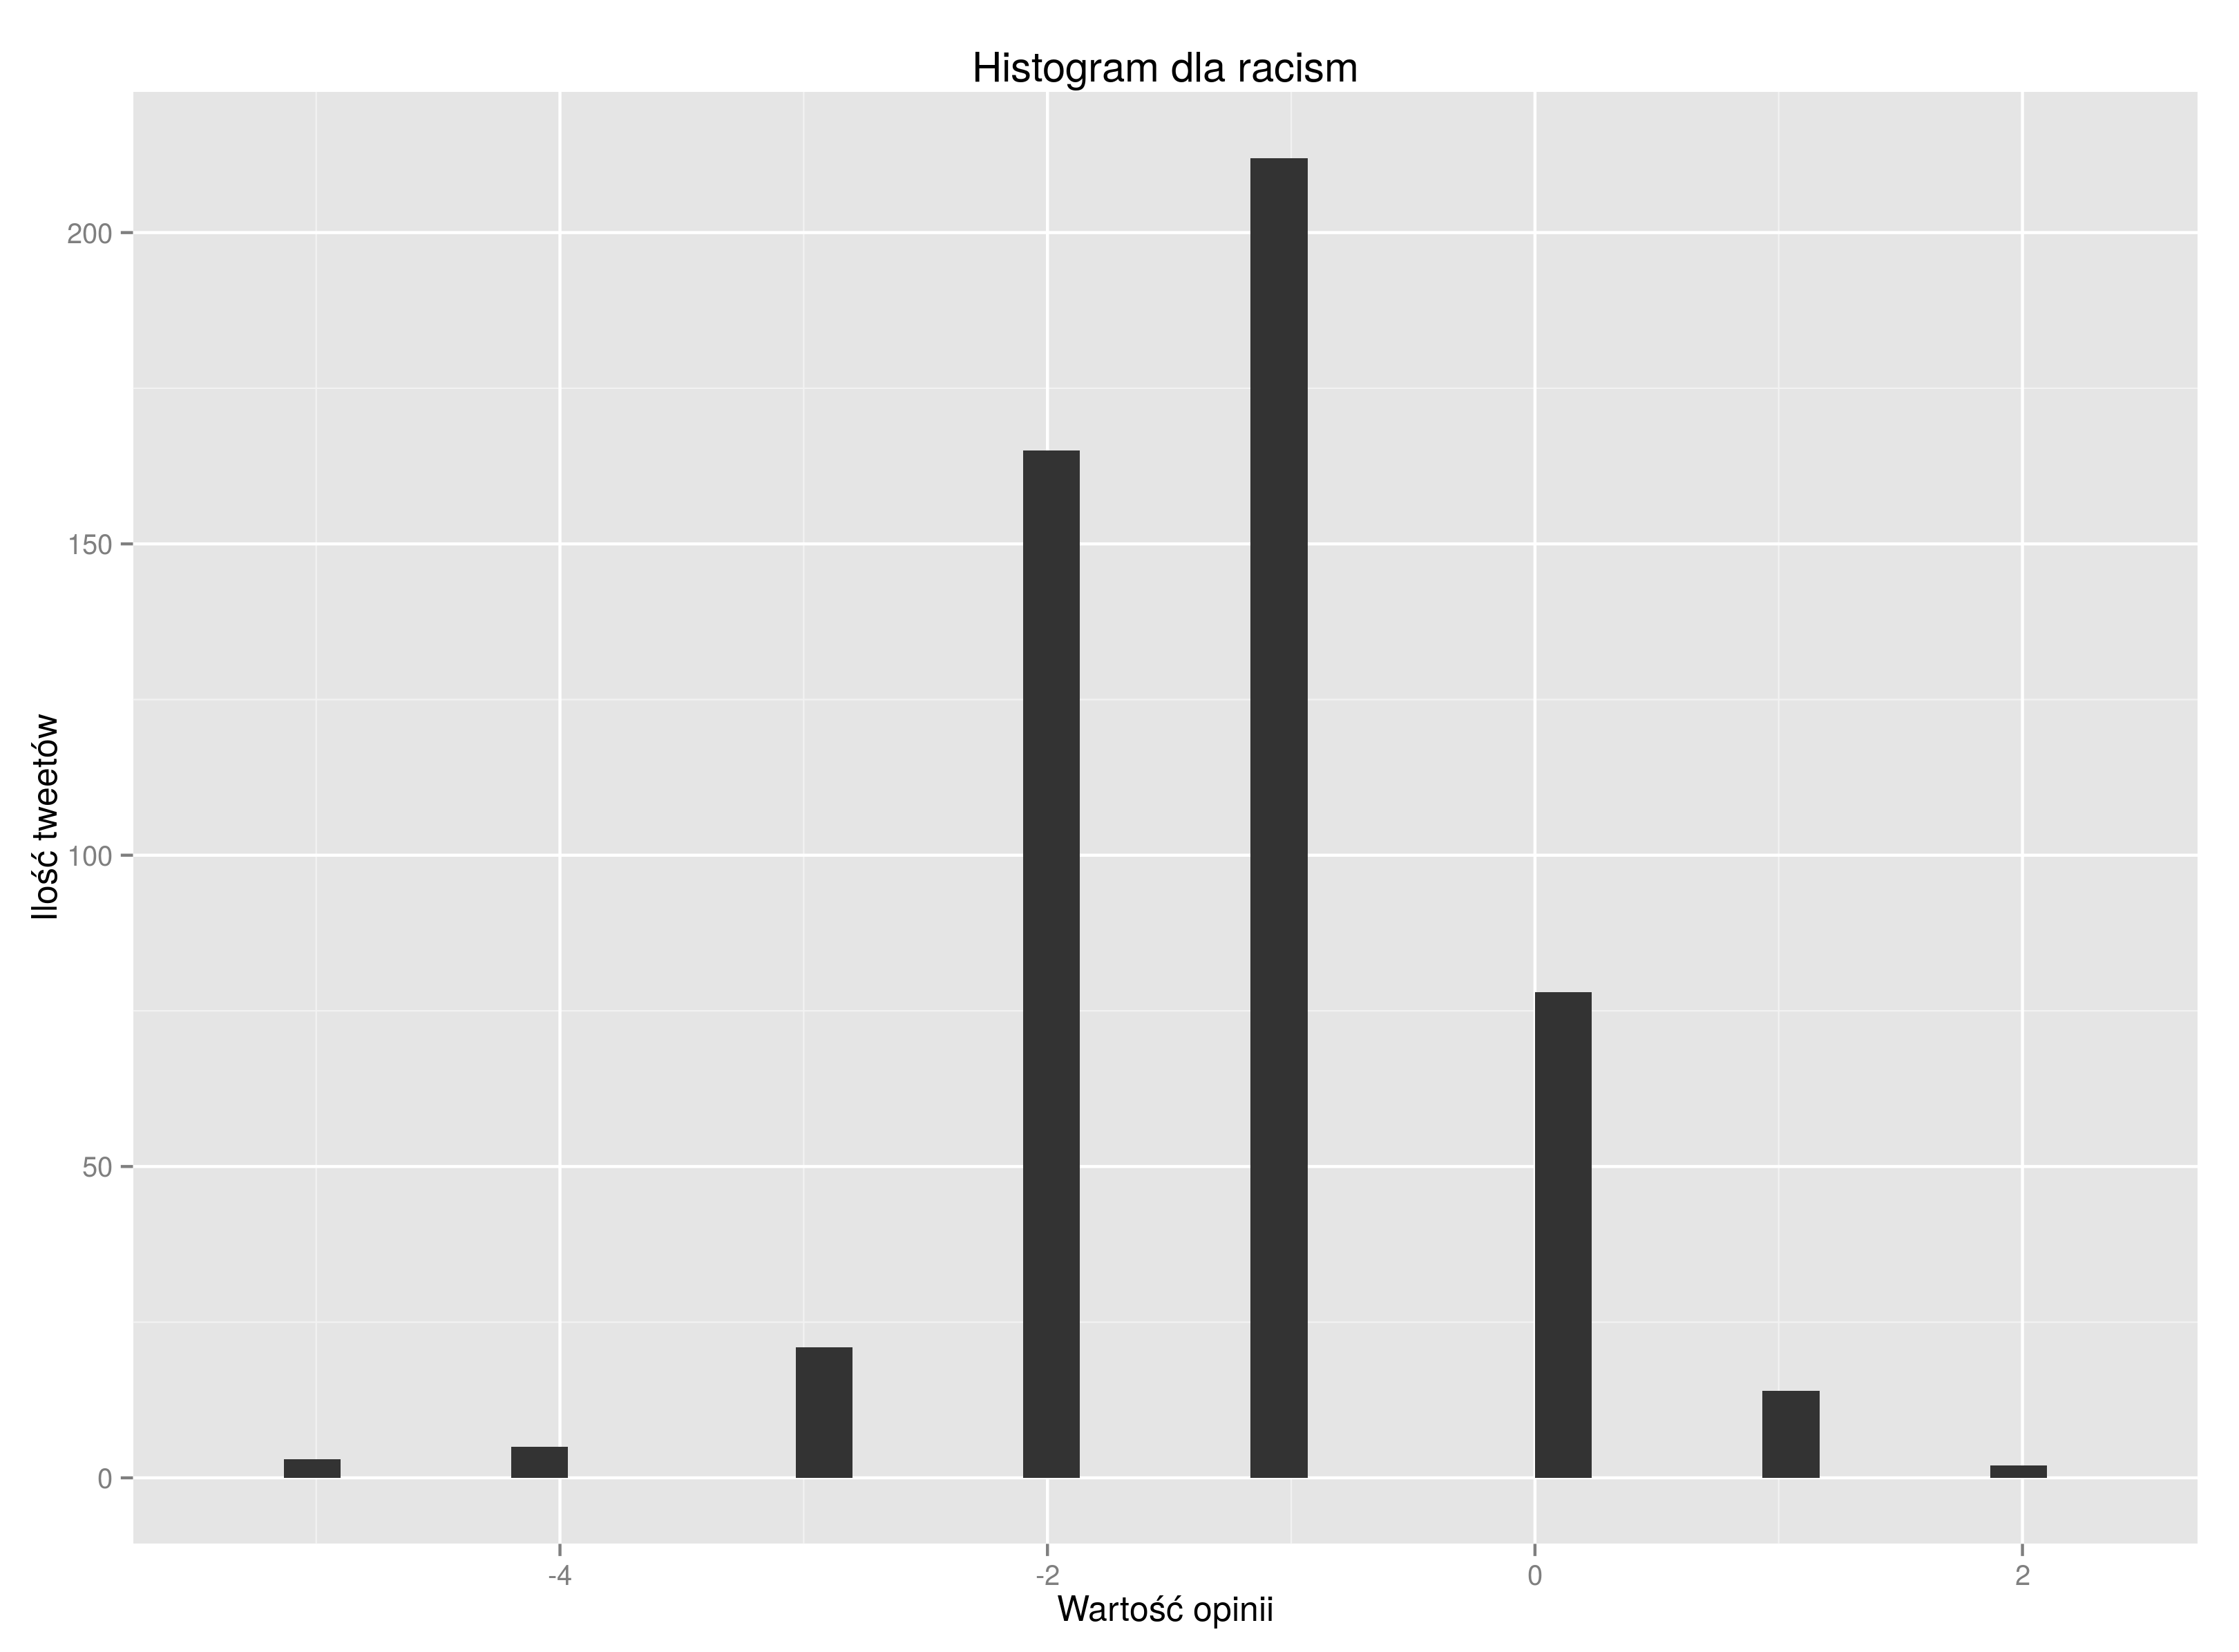
\includegraphics[scale=0.35]{pictures/Histracism.png}
\end{center}

\begin{center}
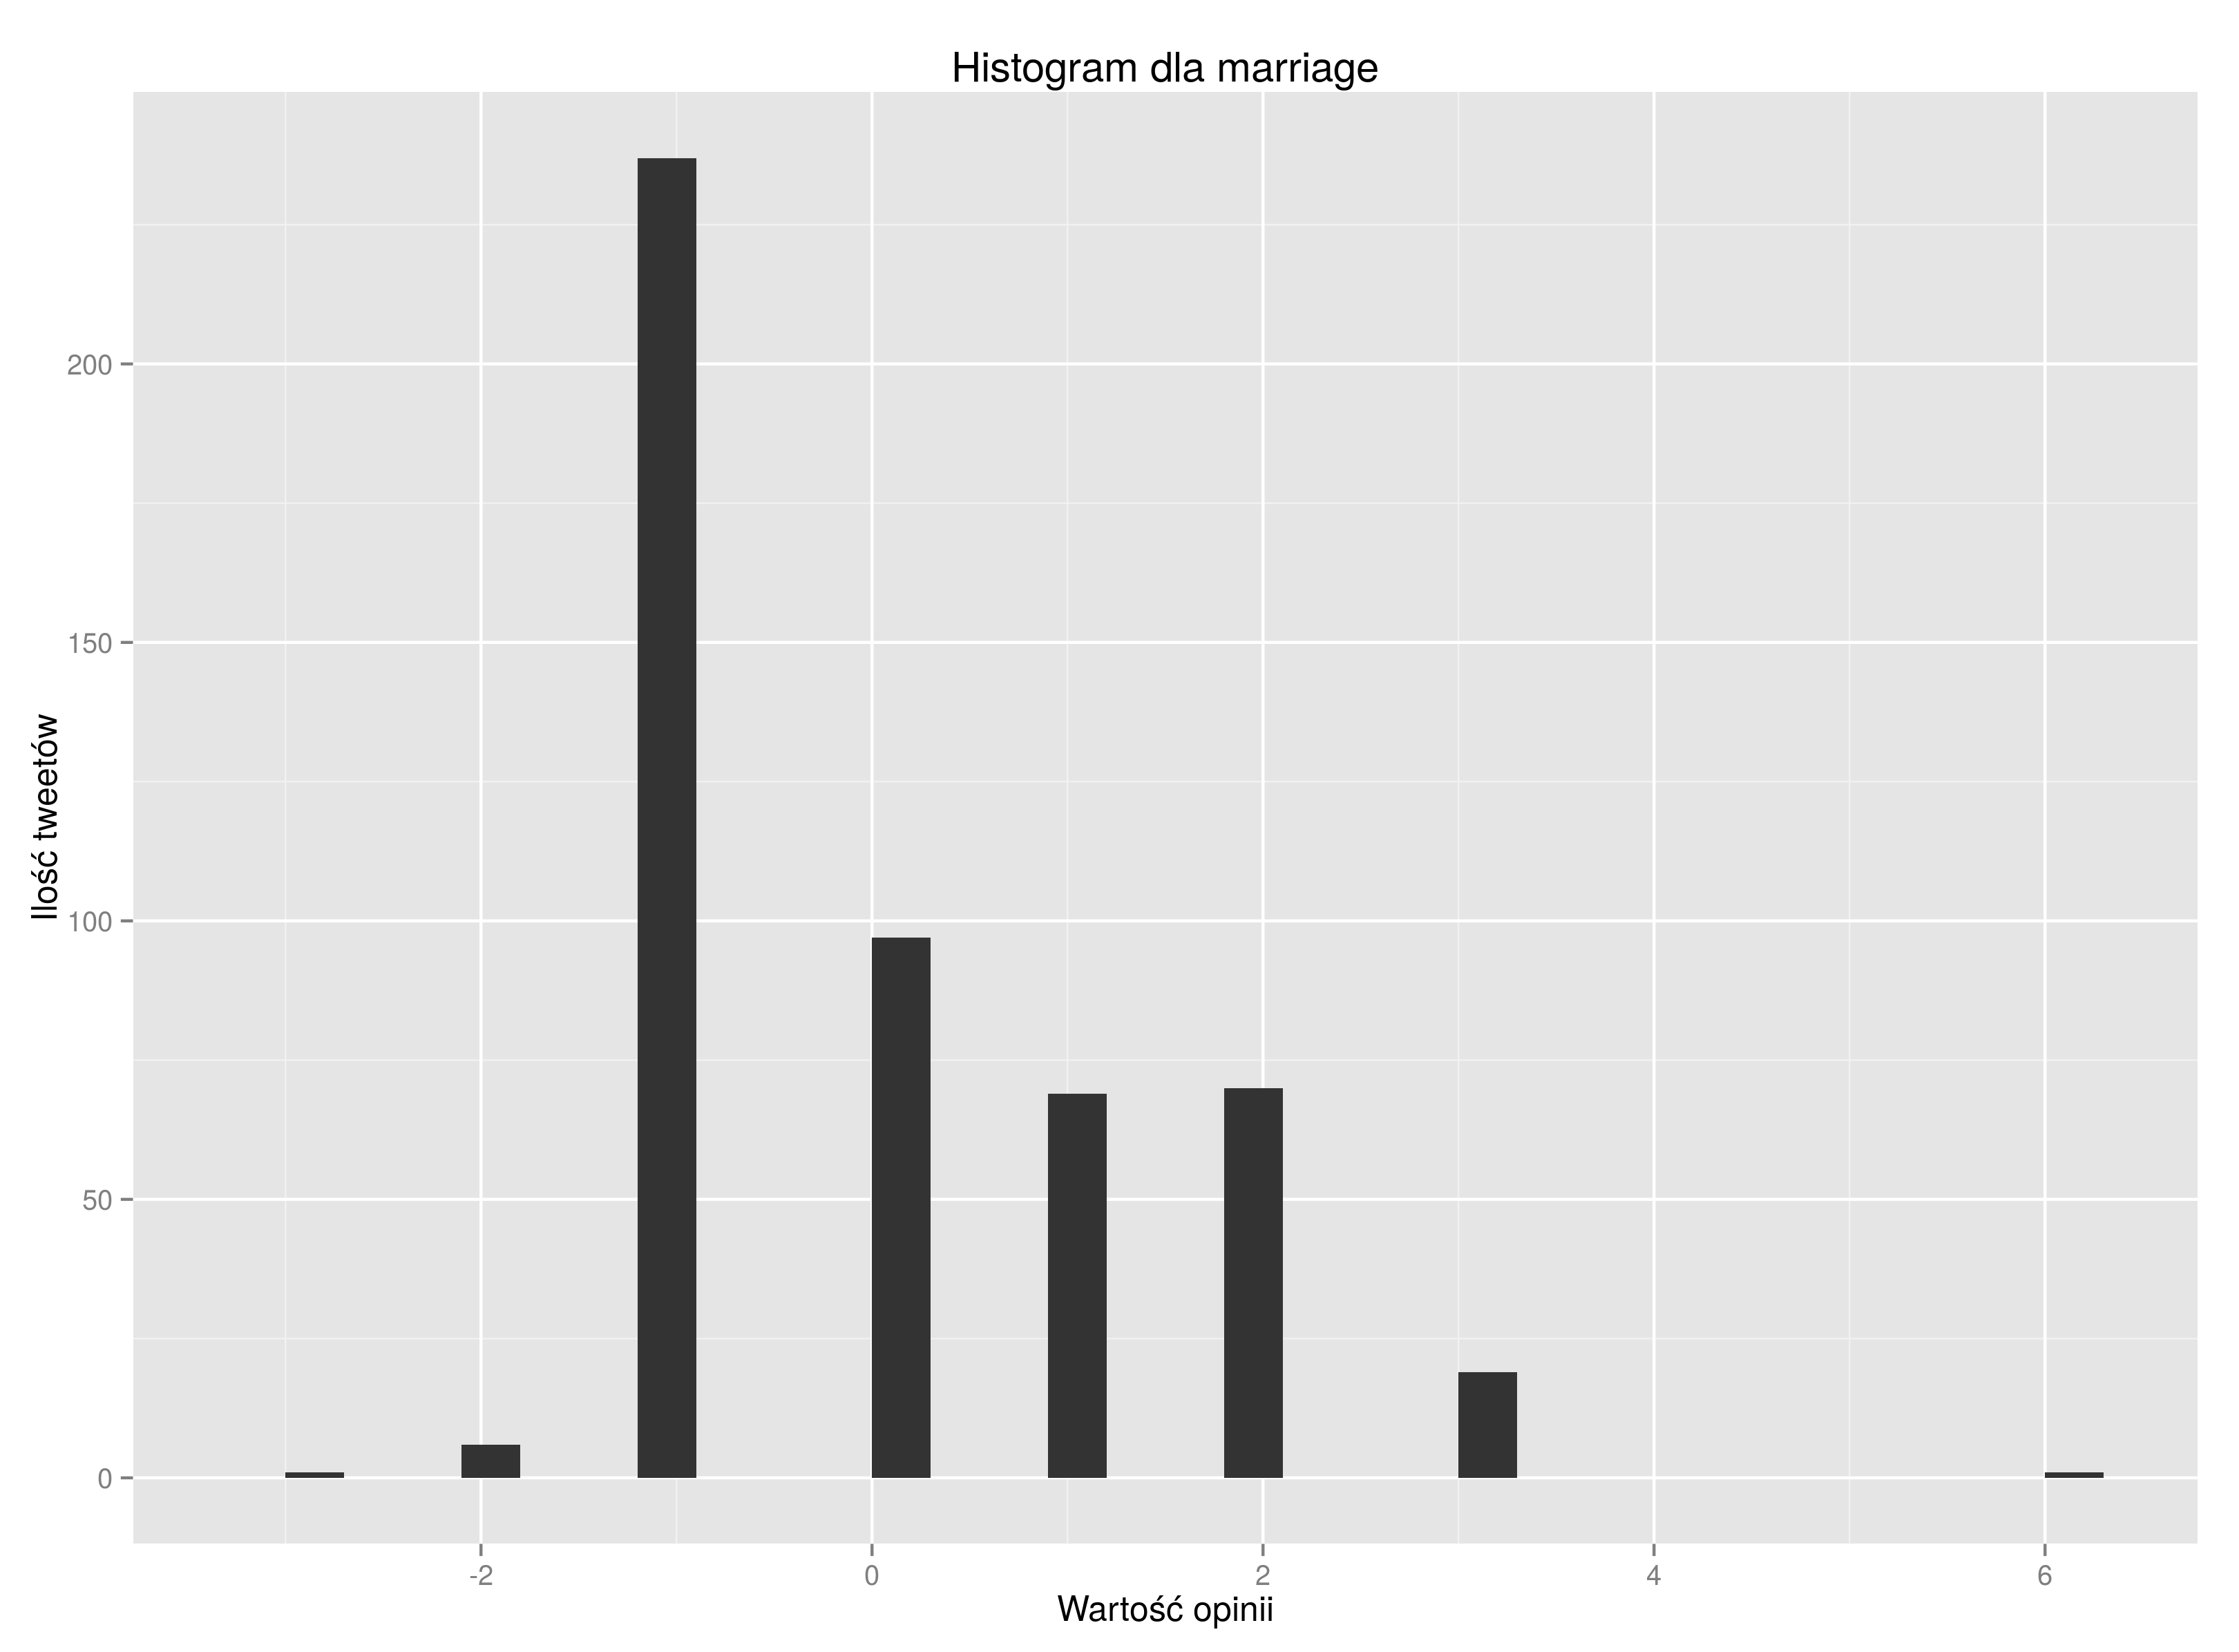
\includegraphics[scale=0.35]{pictures/Histmarriage.png}
\end{center}

\begin{center}
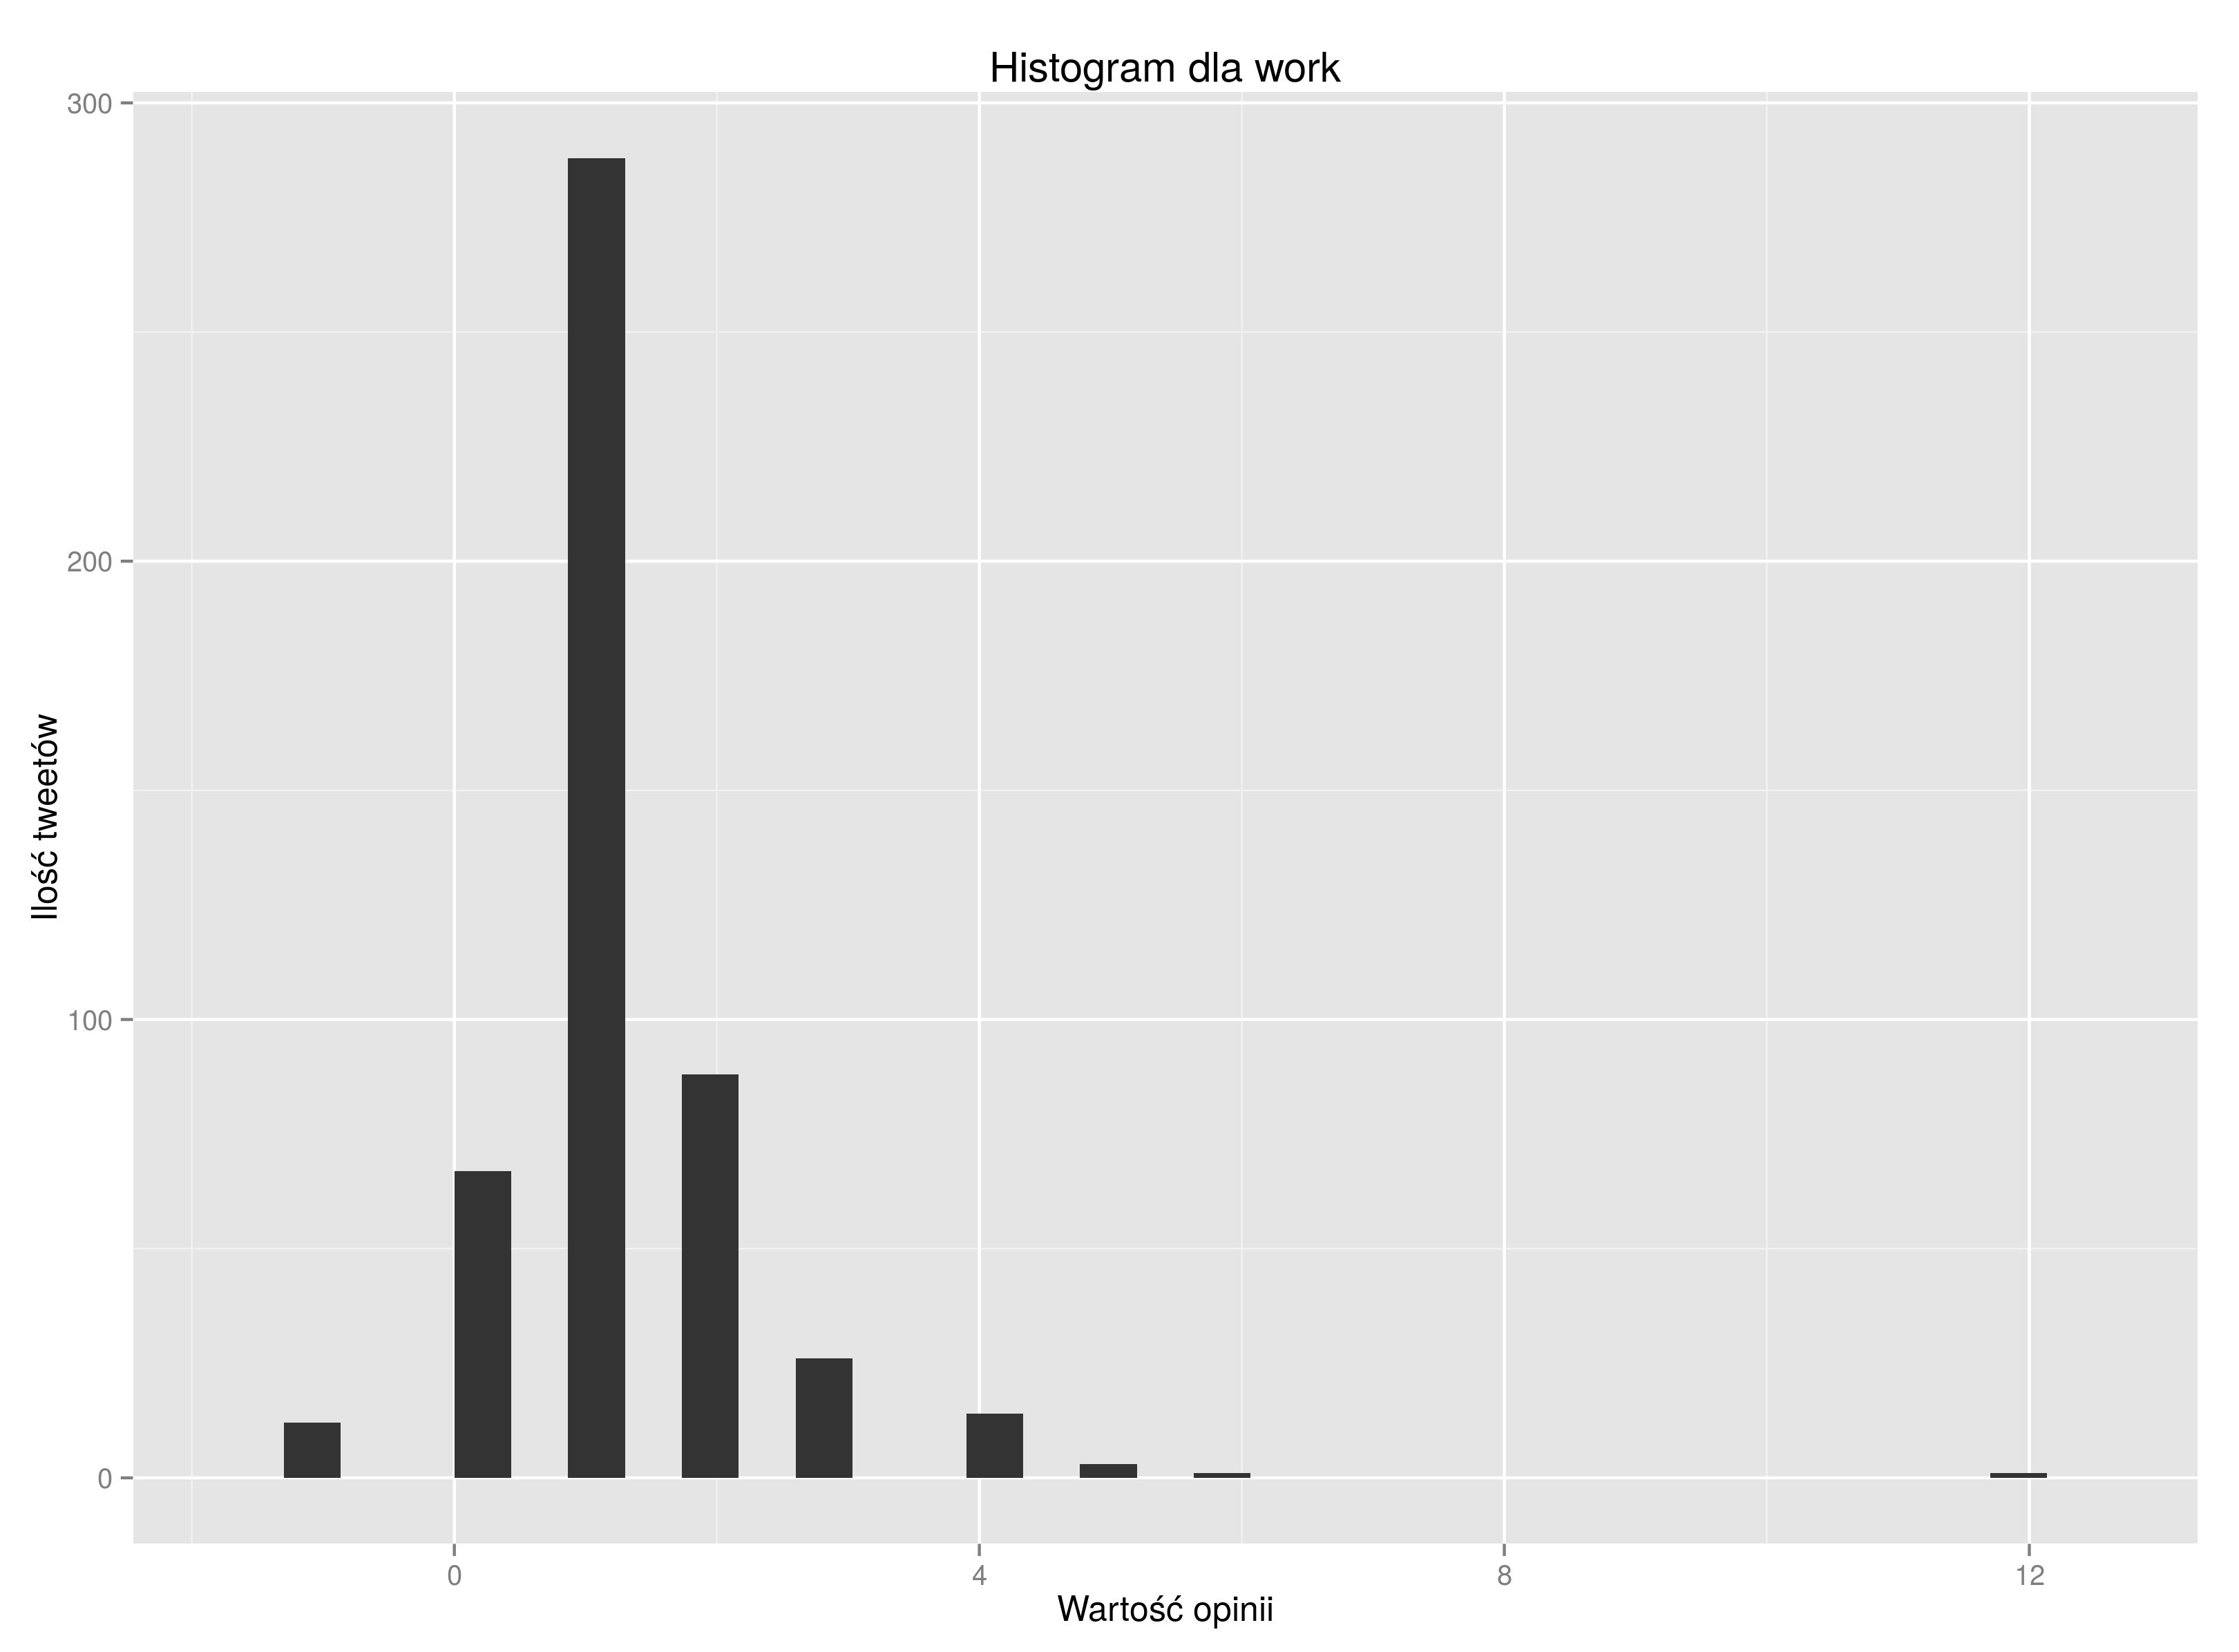
\includegraphics[scale=0.35]{pictures/Histwork.png}
\end{center}

\begin{center}
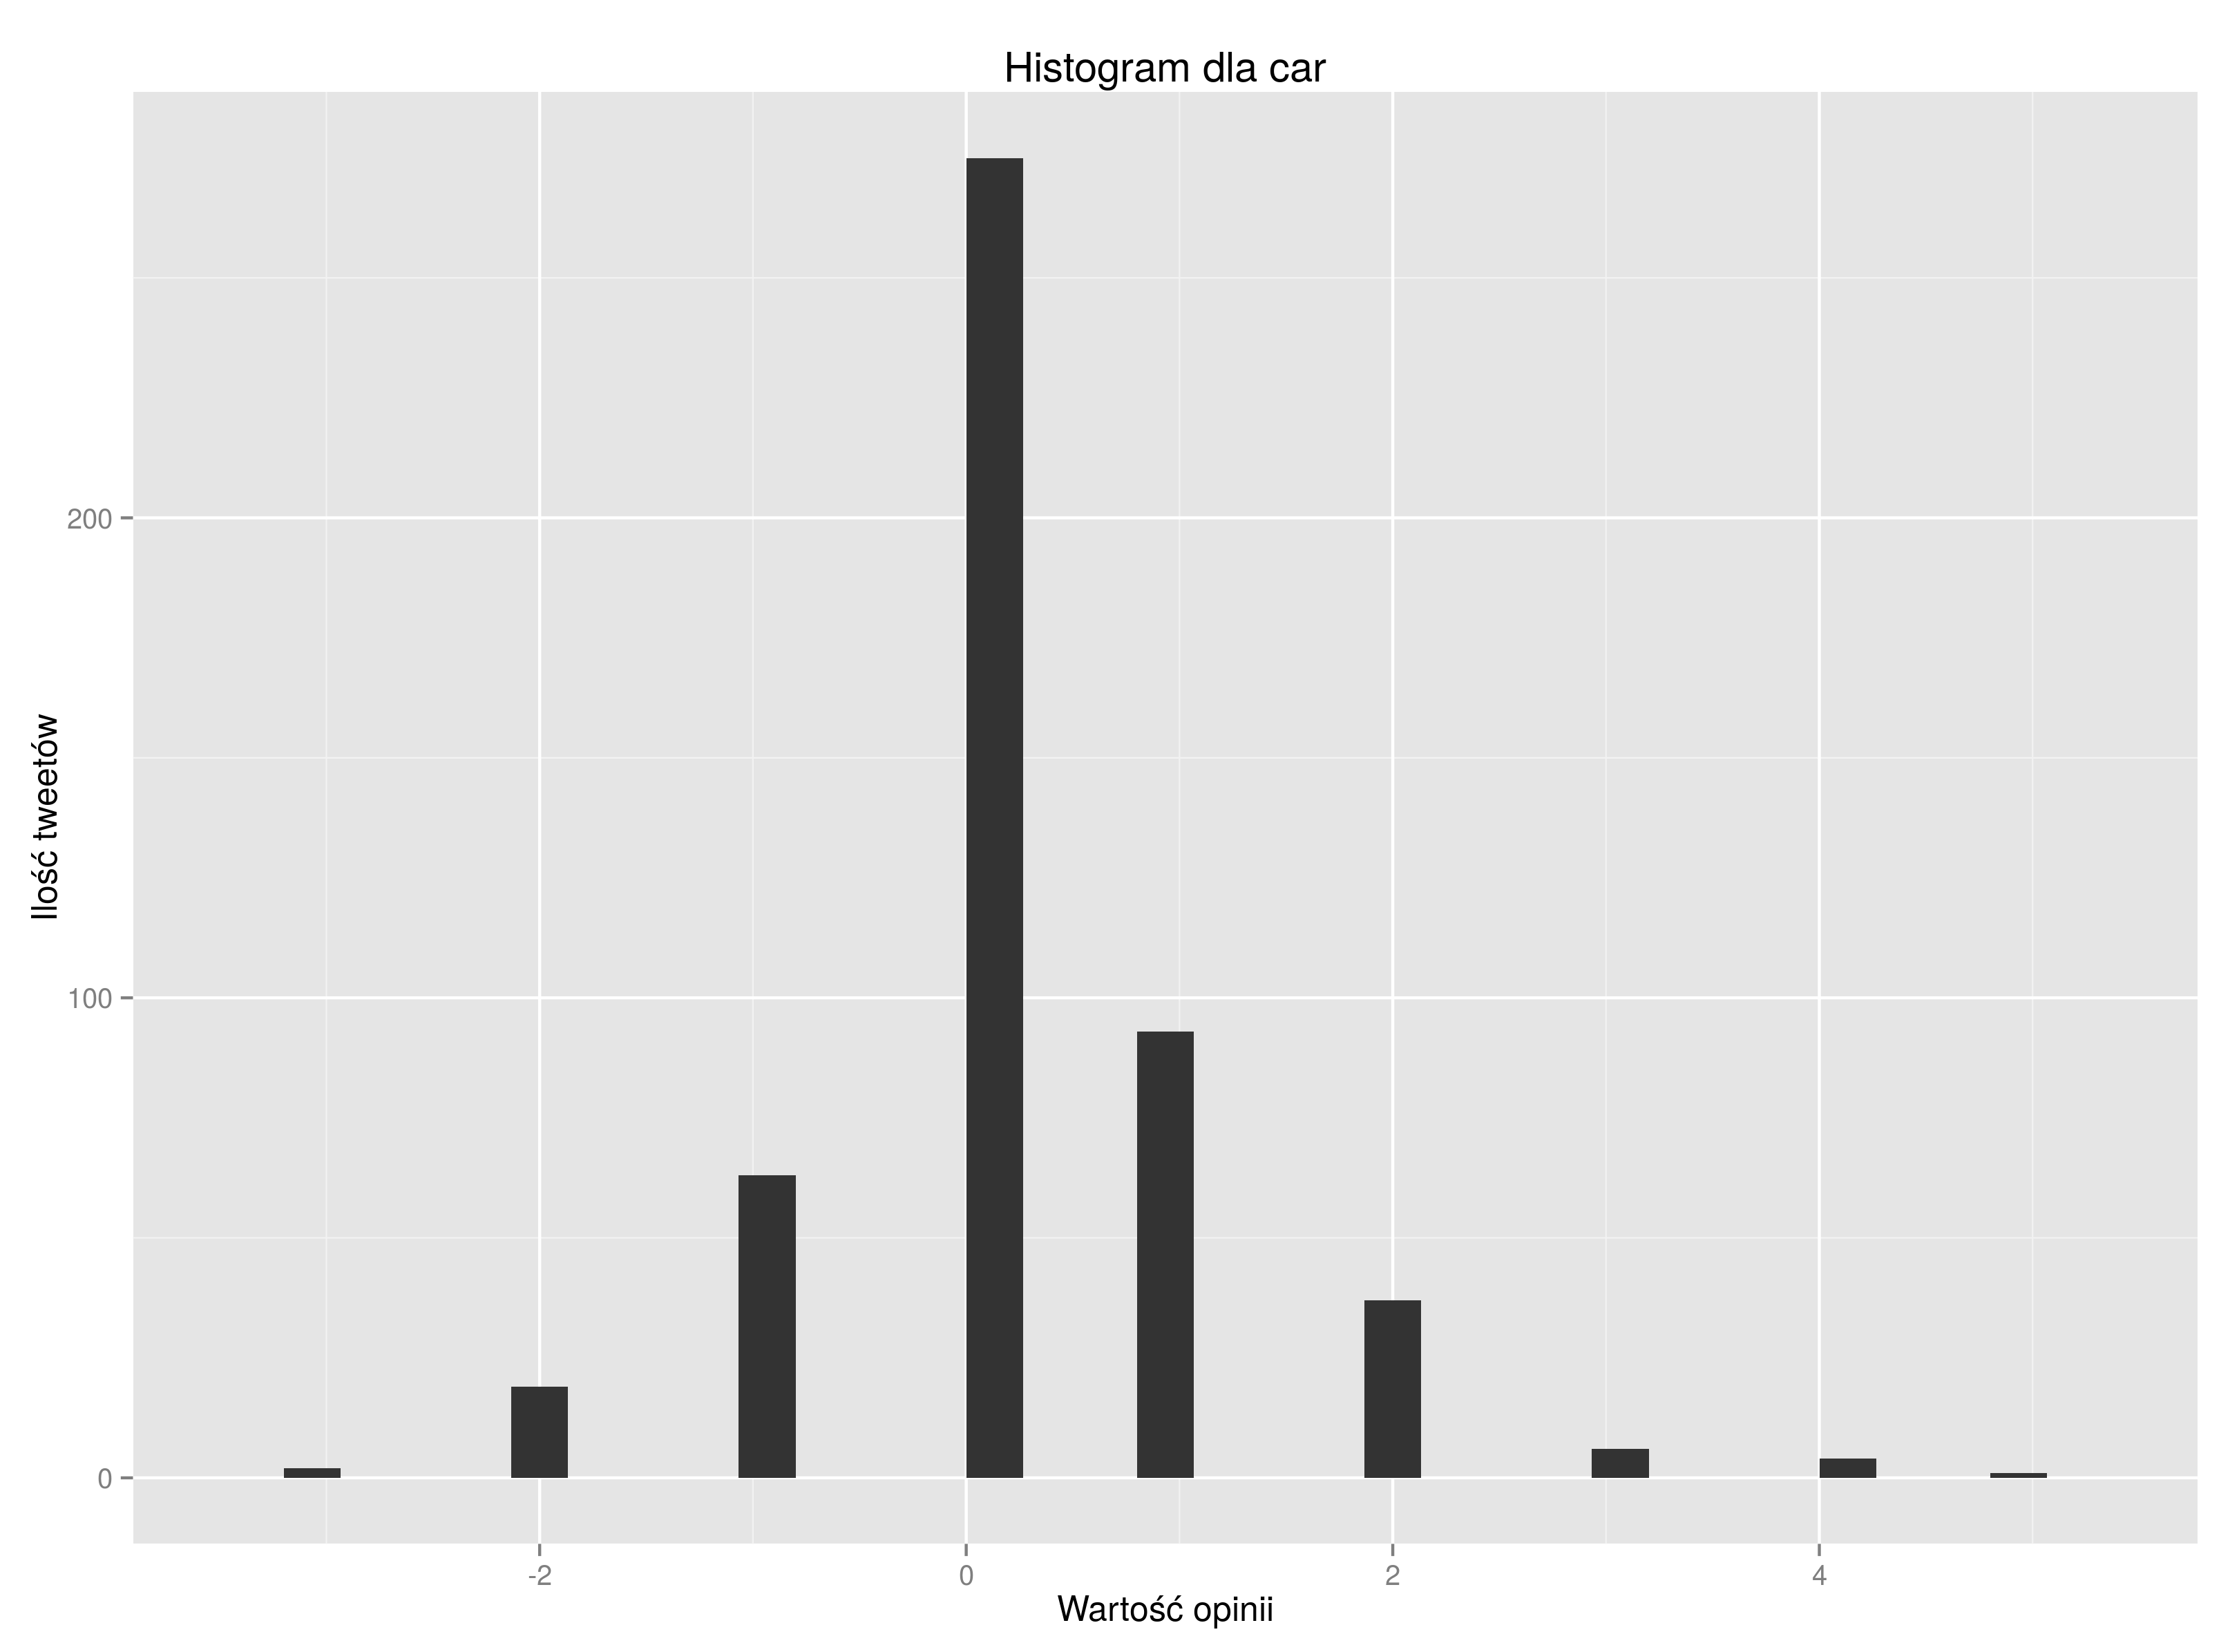
\includegraphics[scale=0.35]{pictures/Histcar.png}
\end{center}

Powyższe wykresy ukazują częstości wartości opinion, który został przydzielony poprzez naszą funkcję sentiment. 

\section[Objaśnienie napisanego programu w języku R] {Objaśnienie napisanego programu w języku R}
\subsection[Ogólne działanie] {Ogólne działanie}
W pełni działający program znajduje się w repozytorium GitHub'a pod adresem: \url{https://github.com/miotek32/DataMiningProject} \\
Program został tak skonstruowany, że wymaga tylko uruchomienia skryptu znajdującego się w pliku \textbf{main.R}. Poza tym jeśli użytkownik chce zmienić dane dla którego chce obliczyć sentiment analysis wystarczy tylko zmienić linijkę \textbf{words} w pliku \textbf{main.R}. Resztę czyli pobranie i zapisanie danych skrypt robi automatycznie. Dane wraz z histogranami zapisane są w folderze \textbf{Data}. Pliki z danymi są zapisane w formacie \textbf{.csv} . Każdy z nich zawiera w pierwszej kolumnie wartość opinii a następnie samą opinie, ale w swej pierwotnej postaci.
\subsection[Plik CreateData.R]{Plik CreateData.R}
Plik \textbf{CreateData.R} zawiera funkcję createData, która za swoje argumenty przyjmuje hasło, które ma poszukiwać na twitterze oraz liczbę tweetów do pobrania. Jego działanie polega na pobraniu tweetów z serwisu oraz zapisanie ich pod nazwą: \textbf{hasło.csv}.

\subsection[Plik LoadTweets.R]{Plik LoadTweets.R}
Plik \textbf{LoadTweets.R} zawiera dwie funkcję: \textbf{score.sentiment} oraz \textbf{sentimentFunction}. Pierwsza z nich realizuje algorytm sentiment analysis, który został wyjaśniony na początku dokumentu. Druga funkcja, która za argument przyjmuje nazwę pliku otwiera ten plik oraz wywołuje funkcję \textbf{score.sentiment} i zapisuje wynik w tym samym pliku. Poza tym generuje on histogram w postaci \textbf{Histhasło.png} oraz wyświetla w konsoli wartości: ilość opinii pozytywnych, negatywnych, neutralnych, średnia oraz odchylenie standardowe.

\subsection[Plik main.R]{Plik main.R}
Główny plik, którego uruchomienie skryptu spowoduje automatyczne wygenerowanie plików, wyświetlenie wartości dotyczącej średniej i odchylenia standardowego oraz wykresu histogramu. Kluczowym elementem w tym pliku jest zmienna words, która zawiera listę słów, które chcemy wykonać algorytm sentiment analysis. 

\section[Ograniczenia] {Ograniczenia}
Pakiet \textbf{twitteR} w języku R ma pewne ograniczenie, które wynika z wykorzystania zewnętrznego API usługi twitter. Polega ona na tym, że niekoniecznie możemy uzyskać żądaną liczbę tweetów dla danego słowa. Bardzo często zdarza się że funkcja \textbf{searchTwitter$($słowo,n=1000$)$} może wyświetlić nam komunikat, że niestety żądaliśmy 1000 tweetów, ale jedynie udało się uzyskać mniejszą ilość. Jest to spowodowane ograniczeniami, które znajdują się w API serwisu twitter. Drugim ograniczeniem jest czas działania programu. Ponieważ język R jest jednowątkowy to wykonanie napisanego tutaj programu trwa około 2 minut. 

\section[Podsumowanie] {Podsumowanie}
Przedstawione tutaj rozwiązanie nie jest jedyne. Istnieje na przykład metoda, która potrafi oprócz sklasyfikowania opinii jako pozytywna czy negatywna, przydzielić która opinia wyrażona jest przez szcześcię, złość itd. Pakiet R posiada takie rozwiązanie, które zawarte jest w pakietach: \textbf{tm} oraz \textbf{sentiment}. Jednak pakiety te są w fazie testowej, nie są one wydane w wersjach produkcyjnych, ale możliwości ich są obiecujące. 

\newpage

\begin{thebibliography}{1}
\bibitem{} \url{http://davetang.org/muse/2013/04/06/using-the-r_twitter-package/}  
\bibitem{} Video kurs: P.Anderson \em{How to use R in Mining Twitter}
\bibitem{} \url{http://www.cs.uic.edu/~liub/FBS/sentiment-analysis.html}
\bibitem{} \url{http://www.regular-expressions.info/posixbrackets.html}
\bibitem{} \url{http://www.r-project.org/}
\bibitem{} \url{http://cran.r-project.org/web/packages/available_packages_by_name.html}
\end{thebibliography}


\end{document}